%
% jacobi.tex
%
% (c) 2024 Prof Dr Andreas Müller
%
\begin{figure}
\centering
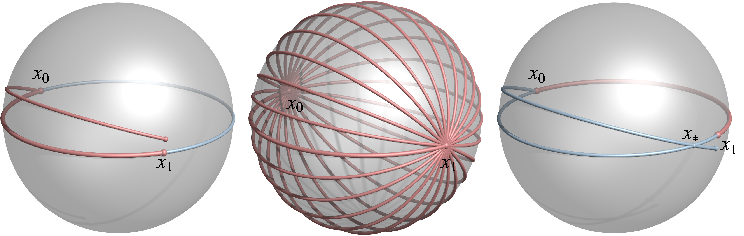
\includegraphics{chapters/060-variation2/images/jacobi.pdf}
\caption{Extremalen und Nullstellen der Jacobi-Differentialgleichung
auf einer Kugeloberfläche.
a) Wenn die Jacobi-Differentialgleichung im Intervall $[x_0,x_1]$ keine
Nullstellen hat, liegt ein Minimum vor.
b) Wenn die Lösung $u_0(x)$ im Punkt $x_1$ verschwindet, ist die
zweite Variation $\delta^2 I(y)\ge 0$ und verschwindet für $\eta = u_0$.
c) Wenn $x_*\in[x_0,x_1]$ eine Nullstelle der Jacobi-Differentialgleichung
ist, dann liegt kein Minimum vor.
Das Minimum wird stattdessen vom roten Teil des Grosskreises auf der anderen
Seite der Kugel angenommen.
Der konjugierte Punkt $x_*$ ist der Antipodenpunkt von $x_0$.
\label{buch:variation2:fig:jacobi}}
\end{figure}
